% Options for packages loaded elsewhere
\PassOptionsToPackage{unicode}{hyperref}
\PassOptionsToPackage{hyphens}{url}
%
\documentclass[
]{book}
\usepackage{amsmath,amssymb}
\usepackage{lmodern}
\usepackage{ifxetex,ifluatex}
\ifnum 0\ifxetex 1\fi\ifluatex 1\fi=0 % if pdftex
  \usepackage[T1]{fontenc}
  \usepackage[utf8]{inputenc}
  \usepackage{textcomp} % provide euro and other symbols
\else % if luatex or xetex
  \usepackage{unicode-math}
  \defaultfontfeatures{Scale=MatchLowercase}
  \defaultfontfeatures[\rmfamily]{Ligatures=TeX,Scale=1}
\fi
% Use upquote if available, for straight quotes in verbatim environments
\IfFileExists{upquote.sty}{\usepackage{upquote}}{}
\IfFileExists{microtype.sty}{% use microtype if available
  \usepackage[]{microtype}
  \UseMicrotypeSet[protrusion]{basicmath} % disable protrusion for tt fonts
}{}
\makeatletter
\@ifundefined{KOMAClassName}{% if non-KOMA class
  \IfFileExists{parskip.sty}{%
    \usepackage{parskip}
  }{% else
    \setlength{\parindent}{0pt}
    \setlength{\parskip}{6pt plus 2pt minus 1pt}}
}{% if KOMA class
  \KOMAoptions{parskip=half}}
\makeatother
\usepackage{xcolor}
\IfFileExists{xurl.sty}{\usepackage{xurl}}{} % add URL line breaks if available
\IfFileExists{bookmark.sty}{\usepackage{bookmark}}{\usepackage{hyperref}}
\hypersetup{
  pdftitle={Porque quise},
  pdfauthor={Fumiko Kaneko},
  hidelinks,
  pdfcreator={LaTeX via pandoc}}
\urlstyle{same} % disable monospaced font for URLs
\usepackage{longtable,booktabs,array}
\usepackage{calc} % for calculating minipage widths
% Correct order of tables after \paragraph or \subparagraph
\usepackage{etoolbox}
\makeatletter
\patchcmd\longtable{\par}{\if@noskipsec\mbox{}\fi\par}{}{}
\makeatother
% Allow footnotes in longtable head/foot
\IfFileExists{footnotehyper.sty}{\usepackage{footnotehyper}}{\usepackage{footnote}}
\makesavenoteenv{longtable}
\usepackage{graphicx}
\makeatletter
\def\maxwidth{\ifdim\Gin@nat@width>\linewidth\linewidth\else\Gin@nat@width\fi}
\def\maxheight{\ifdim\Gin@nat@height>\textheight\textheight\else\Gin@nat@height\fi}
\makeatother
% Scale images if necessary, so that they will not overflow the page
% margins by default, and it is still possible to overwrite the defaults
% using explicit options in \includegraphics[width, height, ...]{}
\setkeys{Gin}{width=\maxwidth,height=\maxheight,keepaspectratio}
% Set default figure placement to htbp
\makeatletter
\def\fps@figure{htbp}
\makeatother
\setlength{\emergencystretch}{3em} % prevent overfull lines
\providecommand{\tightlist}{%
  \setlength{\itemsep}{0pt}\setlength{\parskip}{0pt}}
\setcounter{secnumdepth}{5}
\usepackage{booktabs}
\ifluatex
  \usepackage{selnolig}  % disable illegal ligatures
\fi
\usepackage[]{natbib}
\bibliographystyle{apalike}

\title{Porque quise}
\author{Fumiko Kaneko}
\date{01/01/2020}

\begin{document}
\maketitle

{
\setcounter{tocdepth}{1}
\tableofcontents
}
\hypertarget{section}{%
\chapter*{}\label{section}}
\addcontentsline{toc}{chapter}{}

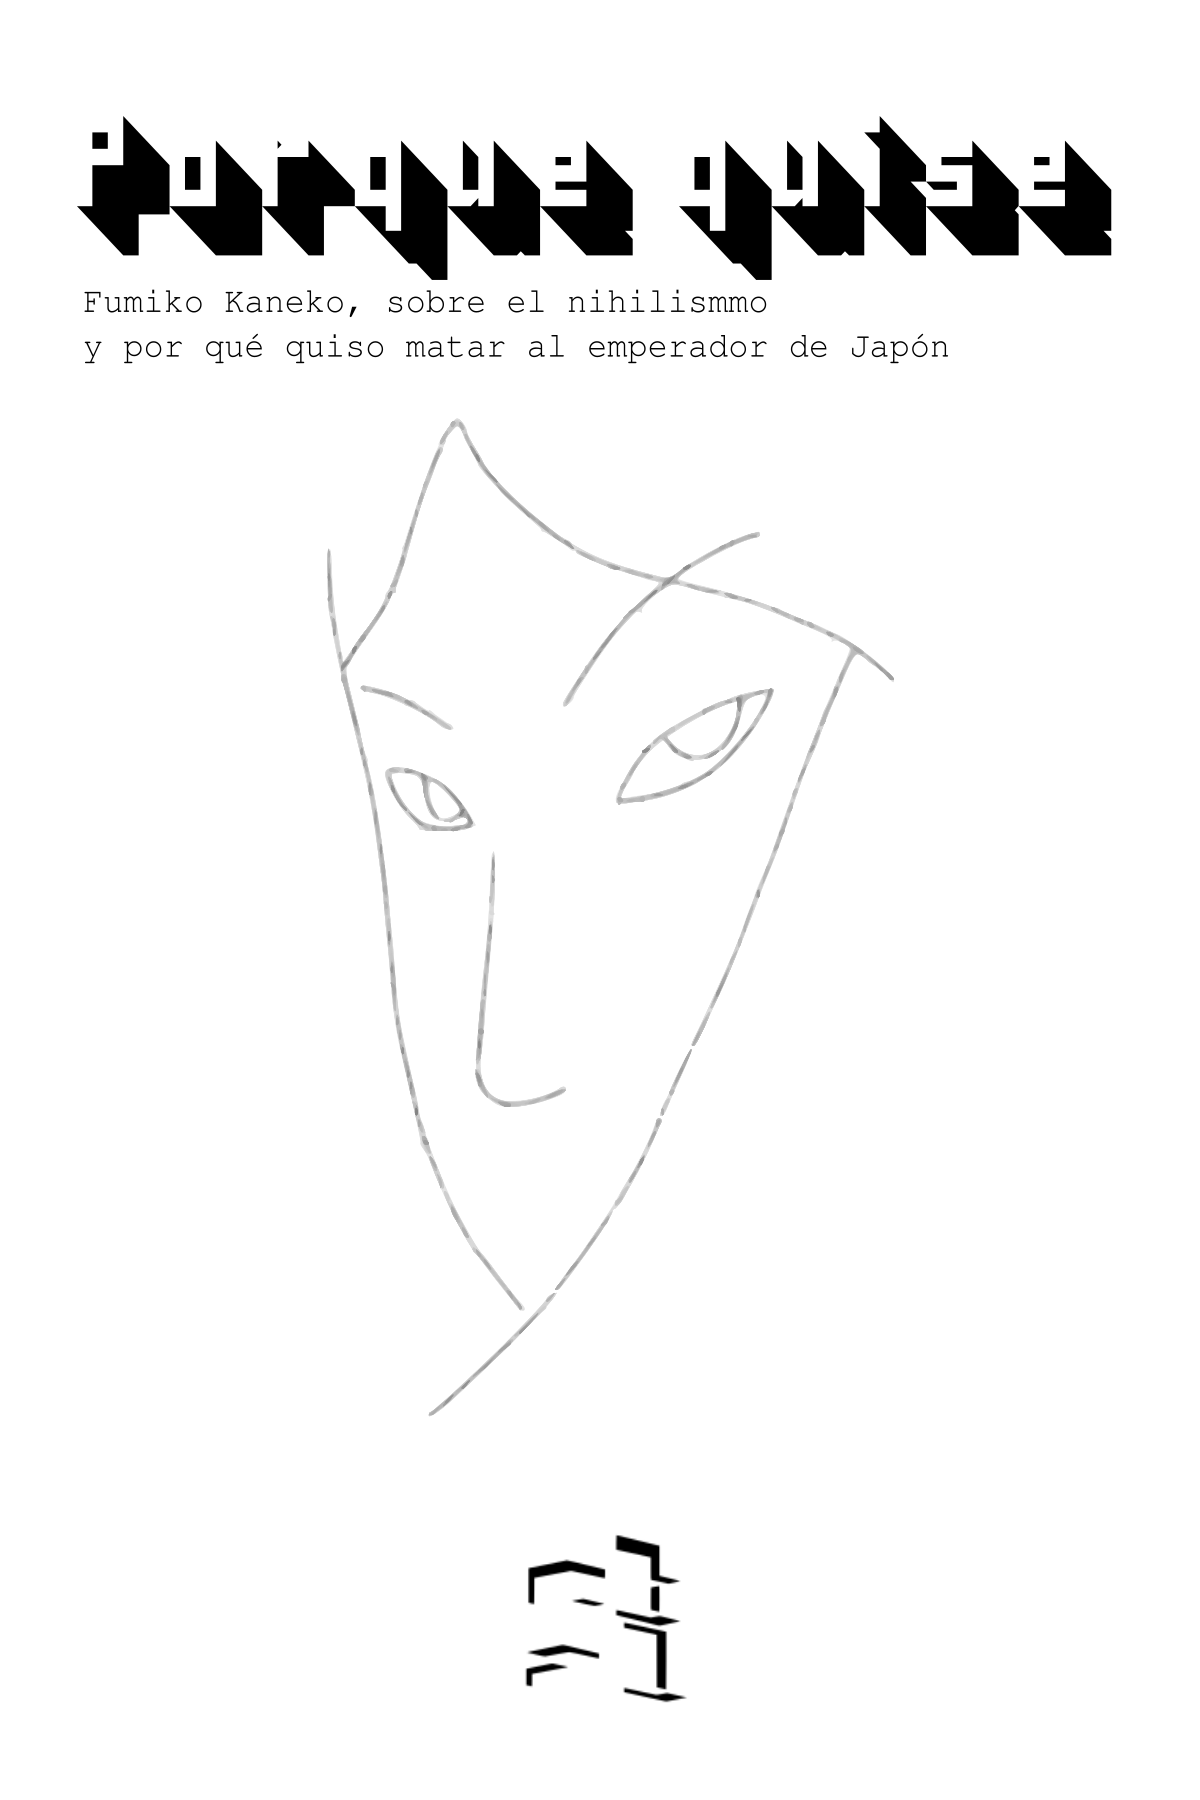
\includegraphics{images/pqq2.png}

Kaneko, Fumiko

Porque quise / 1a ed.~- Ciudad Interdimensional de
Buenos Aires: etal, 2021.

Compilación: Max Res

Traducción, revisión, diseño y maquetado: alf

Título original: \href{https://theanarchistlibrary.org/library/max-res-kaneko-fumiko-because-i-wanted-to}{\emph{Because I wanted to}.}

\begin{figure}
\centering

\includegraphics{images/lccc.png}
\caption{🄯2020 - etal. El texto de esta publicación y esta edición se liberan bajo la Licencia de
Producción de Pares}
\end{figure}

\hypertarget{licencia-de-producciuxf3n-de-pares-versiuxf3n-legible-por-humanes}{%
\chapter*{Licencia de Producción de Pares (Versión legible por humanes)}\label{licencia-de-producciuxf3n-de-pares-versiuxf3n-legible-por-humanes}}
\addcontentsline{toc}{chapter}{Licencia de Producción de Pares (Versión legible por humanes)}

\begin{quote}
Esto es un resumen legible por humanos del \href{http://endefensadelsl.org/ppl_es.html}{texto legal (la licencia
completa)}
\end{quote}

\hypertarget{ud.-es-libre-de}{%
\section*{Ud. es libre de}\label{ud.-es-libre-de}}
\addcontentsline{toc}{section}{Ud. es libre de}

\begin{itemize}
\tightlist
\item
  Compartir - copiar, distribuir, ejecutar y comunicar públicamente la obra
\item
  Hacer obras derivadas
\end{itemize}

\hypertarget{bajo-las-condiciones-siguientes}{%
\section*{Bajo las condiciones siguientes:}\label{bajo-las-condiciones-siguientes}}
\addcontentsline{toc}{section}{Bajo las condiciones siguientes:}

\begin{figure}
\centering

\includegraphics{images/by.png}
\caption{\textbf{Atribución} - Debe reconocer los créditos de la obra de la manera
especificada por el autor o el licenciante (pero no de una manera que sugiera
que tiene su apoyo o que apoyan el uso que hace de su obra).}
\end{figure}

\begin{figure}
\centering

\includegraphics{images/sa.png}
\caption{\textbf{Compartir bajo la Misma Licencia} - Si altera o transforma esta obra, o
genera una obra derivada, sólo puede distribuir la obra generada bajo una
licencia idéntica a ésta.}
\end{figure}

\begin{figure}
\centering

\includegraphics{images/nc.png}
\caption{\textbf{No Capitalista} - La explotación comercial de esta obra sólo está permitida
a cooperativas, organizaciones y colectivos sin fines de lucro, a
organizaciones de trabajadores autogestionados, y donde no existan relaciones
de explotación. Todo excedente o plusvalía obtenidos por el ejercicio de los
derechos concedidos por esta Licencia sobre la Obra deben ser distribuidos por y
entre los trabajadores.}
\end{figure}

\hypertarget{entendiendo-que}{%
\section*{Entendiendo que}\label{entendiendo-que}}
\addcontentsline{toc}{section}{Entendiendo que}

\begin{itemize}
\item
  \textbf{Renuncia} - Alguna de estas condiciones puede no aplicarse si se obtiene
  el permiso del titular de los derechos de autor.
\item
  \textbf{Dominio Público} - Cuando la obra o alguno de sus elementos se halle en
  el dominio público según la ley vigente aplicable, esta situación no quedará
  afectada por la licencia.
\item
  \textbf{Otros derechos} - Los derechos siguientes no quedan afectados por
  la licencia de ninguna manera:

  \begin{itemize}
  \item
    Los derechos derivados de usos legítimos u otras limitaciones
    reconocidas por ley no se ven afectados por lo anterior;
  \item
    Los derechos morales del autor;
  \item
    Derechos que pueden ostentar otras personas sobre la propia obra o
    su uso, como por ejemplo derechos de imagen o de privacidad.
  \end{itemize}
\item
  \textbf{Aviso} - Al reutilizar o distribuir la obra, tiene que dejar muy en claro
  los términos de la licencia de esta obra. La mejor forma de hacerlo es
  enlazar a esta página.
\end{itemize}

\hypertarget{section-1}{%
\chapter*{}\label{section-1}}
\addcontentsline{toc}{chapter}{}

\begin{quote}
Inclinada,

mirando a les demás desde abajo

de mis muslos: el estado

del mundo que necesito mirar,

al revés.
\end{quote}

\textbf{Kaneko Fumiko}

\hypertarget{introducciuxf3n}{%
\chapter*{Introducción}\label{introducciuxf3n}}
\addcontentsline{toc}{chapter}{Introducción}

Kaneko Fumiko (1903-1926) fue una anarquista japonesa que vivió a principios del siglo XX. Nacida ilegitimamente y en una pobreza extrema, vivió su vida como una paria en la sociedad japonesa, incluyendo un periodo en que vivió en la entonces ocupada Corea bajo la tutela de parientes que cuando no indiferentes, fueron crueles con ella. Sus experiencias inspiraron tanto su rebelión contra la autoridad, como sus sentimientos de solidaridad con tode aquelle marginade de la sociedad. Junto a su amigo, pareja y antes de su muerte, esposo, Pak Yol, inició sociedades anarquistas clandestinas; publicó artículos contra el estado y la sociedad del Japón imperial y tal vez, planificó matar al emperador Taisho y al entonces príncipe heredero Hirohito el día de su casamiento.

Ella y Pak eran algunes de les muches que serían arrastrades por los arrestos y asesinatos masivos de enemigues del estado, tanto reales como percibides después del \href{https://es.wikipedia.org/wiki/Gran_terremoto_de_Kant\%C5\%8D}{Gran Terremoto de Kanto de 1923}. Bajo ``custodia protectora'', ella y Pak fueron juzgades y condenades a muerte por alta traición en cargos relacionados con un complot para matar al emperador y al príncipe heredero. Si bien estas sentencias fueron conmutadas posteriormente a cadena perpetua por el emperador, Fumiko rechazó este honor rápidamente al romper el decreto en la cara de sus carceleros. Poco tiempo después, en 1926, la encontraron colgada en su celda, por lo que se difundió que había cometido suicidio.

Estas transcripciones de los interrogatorios de Fumiko Kaneko proporcionan una mirada valiosa a sus pensamientos y a los hechos de su vida más allá de la época de su juventud detallada en \emph{The Prison Memoirs of a Japanese Woman}, una memoria que escribió durante su juicio. En algunos momentos la vemos discutiendo sus filosofías sobre el nihilismo y la individualidad, el dualismo, la influencia de Stirner que se asoma en su protesta contra el ``fantasma'' del altruismo confuciano y la insistencia de que les marginades deberíamos ser el centro de todas las cosas. Sus denuncias al emperador y al estado japonés también son conmovedoras aunque la esencia del complot para el asesinato que presenta fuertemente en el segundo interrogatorio incluido acá es bastante confuso porque, como observa Helene Bowen Raddeker (1997), durante sus interrogatorios probablemente habría inflado su papel para parecer más culpable y ser sentenciada tan severamente como Pak. De esta forma, aunque en la primera entrevista de 1925 (tambien presentada en esta publicación) habla de un intento fallido de Pak para conseguirle explosivos en Corea, más tarde, en 1926, se desmiente y admite que se enteró del intento de Pak solo después de que éste volviera de Corea\footnote{Raddeker, Helene Bowen. \emph{Treacherous Women of Imperial Japan: Patriarchal Fictions, Patricidal Fantasies}. Routledge, 1997.}. Sin embargo, trasladó su réplica al sistema imperial japonés al trato con los interrogadores de forma tan feroz que la mantuvieron en la carcel, incluso después de dicha admisión.

Este panfleto incluye tres interrogatorios: el primero está extraído de \emph{Reflections on the Way to the Gallows} (``Reflexiones en el Camino a la Horca'') de Hane Mikiso que incluye el testimonio de Fumiko Kaneko sobre cómo llegó a dar con su filosofía nihilista, así como la denuncia al sistema imperial japonés y al emperador; el segundo y el tercer interrogatorio, traducidos por Max Res, tienen lugar dos años más tarde que el primero y fueron extraídos por Kurihara Yasushi en su compilación de escritos anarquistas japoneses, \emph{Kurizake}, (``Libertad''). Estos incluyen denuncias más contundentes al emperador y a la sociedad japonesa. Aparte de estos textos existe una transcripción completa de los juicios, correspondencias e interrogatorios de Fumiko y Pak en registros judiciales que también se han publicado pero que actualmente están fuera de nuestro alcance. También existen algunos escritos de Fumiko previos al juicio, aunque en un número limitado, y prácticamente todo esto, con la excepción de \emph{The Prison Memoirs of a Japanese Woman}, sigue sin traducirse.

Además de \emph{The Prison Memoirs of a Japanese Woman}, hay otros recursos en inglés para obtener más información sobre Fumiko, que incluyen las mencionadas \emph{Reflections on the Way to the Gallows}, que contiene una traducción de su ensayo \emph{Nani ga watakushi o kō saseta k}" (``Qué me llevo a hacer lo que hice'').

\emph{Treacherous Women of Imperial Japan} de Radikker relata y analiza las historias de Fumiko y Kanno Suga, otra anarquista japonesa ejecutada 15 años antes bajo el cargo de traición e incluye un perfil más robusto de la vida de Fumiko. La familiaridad de Raddeker con el anarquismo, Stirner y Nietzsche y el acceso a una amplia variedad de material fuente carga de valor la lectura. El tanka que abre esta publicación también está extraido de allí (Raddeker 232).

Max Res, día de año nuevo de 2020

\hypertarget{de-noviembre-de-1923}{%
\chapter*{22 de noviembre de 1923}\label{de-noviembre-de-1923}}
\addcontentsline{toc}{chapter}{22 de noviembre de 1923}

{[}Los siguientes son extractos del interrogatorio de Kaneko del 22 de noviembre de 1923{]}\footnote{Esta traducción, que incluye paráfrasis y notas a pie de página, se puede encontrar en \emph{Reflections on the Way to the Gallows: Rebel Women in Prewar Japan} de Mikiso Hane.}

Pregunta: ¿Por qué abrazó el nihilismo?

Respuesta: Por las circunstancias de mi familia y las consiguientes opresiones sociales que sufrí.

P: ¿Y su familia?

R: No tengo familia a decir verdad \ldots{} Mis padres me abandonaron y me separaron de mis hermanos y hermanas. No tuve vida familiar. Mi nacimiento no fue registrado, por lo que toda la vida fui sistemáticamente oprimida por la sociedad. Es culpa del sistema social\ldots{} {[}Después de venir a Tokyo{]} leí los escritos de Toshihiko Sakai y revistas socialistas. Al ver esto, mis padres se preocuparon. Me incliné hacia el socialismo. Aproximadamente en 1922 conocí a un coreano, Pak Yeol, quien era desconocido y carecía de cualquier tipo de propiedad. Decidí vivir con él y puse al tanto a mis padres sobre esto\ldots{} Después de que comencé a vivir con él, mi padre me escribió una carta, en mayo de ese año, alegando que yo era descendiente de un canciller del reino, Fujiwara-no-Fusame {[}681-737{]} que había vivido hace más de cien generaciones. Me dijo que estaba mancillando el ilustre linaje de la familia Saeki viviendo con un humilde coreano. De esa forma me hizo saber que me desheredaba y que en adelante no debería pensar en él como mi padre. Entonces fui desheredada por mi padre, que ya me había abandonado. Mi madre también me abandonó\ldots{} Ella incluso en un momento consideró la posibilidad de venderme a como esclava sexual\ldots{} Mis padres no me dieron amor y sin embargo, trataron de obtener todo el beneficio que pudieron a cuesta mío. El suyo fue un amor verdaderamente egoísta, una forma de codicia. Así que yo, objeto de la codicia, no entiendo el significado de la piedad filial. La moral se basa en la relación entre el fuerte y el débil. Esa moralidad es siempre manipulada para servir a la conveniencia de los fuertes. Es decir, el fuerte insiste en preservar su libertad de acción exigiendo la sumisión de los débiles. Desde el punto de vista de los débiles, la moralidad significa un acuerdo que exige la sumisión de une a los fuertes. Este principio moral es común en todas las edades y en todas las sociedades. El objetivo principal de quienes están en el poder es preservar este principio moral el mayor tiempo posible. La relación entre padres e hijes también está basada en este principio. La expresión ``piedad filial'' sirve para cubrir esa realidad.

P: ¿Cómo llegó a asociarte con les socialistas y finalmente con el nihilismo?

R: Tres grupos intelectuales me influyeron cuando vendía periódicos \ldots{} Uno era un grupo budista de salvación, el segundo fue el grupo del Ejército de Salvación Cristiano y el tercero, los socialistas de pelo largo que gritaban sus consignas con voces desesperadas\ldots{} Primero me acerqué al Ejército de Salvación.

{[}Luego relata sus experiencias con Saitō - identificado en sus memorias como Itō. Explica que se desilusionó con el cristianismo cuando dijo que tenía que terminar su amistad con ella porque se había enamorado de ella{]}.

¡Qué tremenda contradicción para unx cristianx predicar el amor en la esquina de la calle y no darle cabida cuando se presenta en su forma más pura! Les cristianes se encadenaron al concepto de Dios que crearon. La suya es una fe cobarde de esclavxs. La virtud y la belleza del ser humane es vivir de forma natural, sin someternse al gobierno de fuerzas externas. Decidí entonces que no podía abrazar el cristianismo, que predica la doctrina de una vida que entra en conflicto con mis ideales de belleza y virtud. Así que abandoné el cristianismo\ldots{}

{[}Después se hizo amiga de un socialista, Hori Kiyotoshi, pero se desilusionó de él también porque Hori, afirmó, era un hipócrita. Ocultó su relación con su esposa geisha, por temor a que obstaculizara sus posibilidades de salir adelante en el mundo. También hizo que aquelles debajo de él hicieran todo el trabajo en su imprenta, mientras disfrutaba de su tiempo libre{]}.

También me presentaron a otra socialista, Kutsumi Fusako. Su vida familiar y sus principios no eran muy diferentes a los de Hori. Kutsumi se ocupó de sus propias necesidades personales pero no le prestó atención a las necesidades de sus hijes. Siempre encontraba alguna excusa para salir con un hombre joven y quedarse fuera todo el día. Una vez la escuché decir que todo lo que tenía que hacer era subir a una plataforma, dar un discurso sobre el socialismo y decir ``Hay que destruir la sociedad actual'' para provocar una intervención de la policía. Al día siguiente, los periódicos informarían que Kutsumi Fusako dio un discurso extremista, por lo que la policía le impidió hablar. Siempre me disgustó el deseo generalizado entre los socialistas de que sus nombres aparezcan en el periódico. En este momento, Kutsumi no tenía dinero ni siquiera para comprar comida, por lo que empeñó mi ropa sin mi permiso. Luego dejó que el período de rendición expirara y permitió que el empeño se vendiera. No me quejo de perder mi ropa, aunque ella sabía que la necesitaba porque había llegado el invierno. Ella no mostró ningún sentido de responsabilidad. Yo detestaba su actitud, una socialista que supuestamente estaba comprometida con las necesidades ajenas, pero que pensaba solamente en alimentarse a sí misma.

Yo me imaginaba que les socialistas eran personas que se elevaban por encima de las costumbres y la moral sin sentido que impone la sociedad. Les imaginé como luchadores valientes sin interés de inflar su propio ego y la supuesta fama que viene de la reputación social. Pensé que eran guerreres que luchaban para destruir esta sociedad perversa y se esforzaban por crear una distinta. Sin embargo, a pesar de que hacen una denuncia de las injusticias e hipocrecías de la sociedad, y aparentan ser indiferentes a la fama y a la reputación, de hecho se rigen y se preocupan por los estándares vigentes en la sociedad que dicen repudiar. Buscan adornarse con ornamentos convencionales y reproducen los valores convencionales. Así, como los generales se enorgullecen de las medallas condecorativas en sus pechos, les socialistas codician registros de arresto para ganarse el pan. Se enorgullecen de esto. Cuando me di cuenta de este hecho, me alejé.

También llegué a horrorizarme por la somnolencia de les campesines, que están sumides en el dolor pero no sienten dolor, y la ignorancia de les trabajadores, que trabajan diligentemente mientras son devorades hasta los huesos. Si se les quitan las cadenas que les atan, es probable que vayan a los portadores del poder político y económico con sus cadenas a suplicarles que vuelvan a encadenarles. Quizás sean más felices si se les permite simplemente dormir en la ignorancia. Así que me disgusté de todas las corrientes de pensamiento y desde la primavera de 1922 abrazé con fuerza las creencias nihilistas que sostengo hoy.

En cuanto al significado de mi nihilismo \ldots{} en una palabra, es la base de mis pensamientos. El objetivo de mis actividades es la destrucción de todos lo vivo. Siento una ira ilimitada contra la autoridad parental que me aplastó bajo el nombre altisonante del amor paterno, y contra el estado y la autoridad social, que abusó de mí en nombre del amor universal.

Habiendo observado en la realidad social el hecho de que todxs lxs seres vivxs de la tierra están incesantemente comprometidxs en una lucha por la supervivencia, que se matan entre ellxs para sobrevivir, llegué a la conclusión de que si hay un absoluto, una ley universal en la tierra, es la realidad de que los fuertes explotan a los débiles. Esta creo, es la ley y la verdad del universo. Ahora que he visto la verdad sobre la lucha por la supervivencia y el hecho de que los fuertes siempre ganen y los débiles siempre perdamos, no puedo unirme a las filas de les idealistas y adoptar un modo de pensar optimista que sueña con la construcción de una sociedad sin autoridad ni control. Mientras todo lo vivo no desaparezca, las relaciones de poder basadas en el principio de la explotación persistirán. Porque los portadores del poder van a hacer todo lo que esté a su alcance para defender su autoridad de la manera habitual, oprimiendo a los débiles, y porque mi experiencia pasada ha sido una historia de opresión por parte de toda las formas de autoridad decidí negar los derechos reclamados por toda forma de autoridad, rebelarme contra ellos, poniendo en juego no sólo mi propia vida sino la de toda la humanidad en este empeño.
Por esta razón planeé eventualmente lanzar una bomba y aceptar el fin de mi vida. No me importaba si este acto desencadenaba una revolución o no. Estoy perfectamente contenta de satisfacer mis propios deseos. No quiero ayudar a crear una nueva sociedad basada en una nueva forma de autoridad.

P: ¿Cuál es su opinión sobre el sistema estatal y social japonés?

R: Divido el sistema social estatal japonés en tres niveles: la primera clase son los miembros del clan real, la segunda clase son los ministros del gobierno y otros detentores del poder político y la tercera clase son las masas en general.

Considero a la primera clase, el clan real, como víctimas lamentables que viven como presxs, cuyas idas y venidas, al igual que en el caso del regente imperial, están estrictamente reguladas. Pienso que elles son marionetas lamentables y muñecos de madera que están siendo manipulados por la segunda clase, el verdadero portadores del poder, con el fin de poner el velo sobre los ojos de las masas. La tercera clase, la las masas, como mencioné antes, son ignorantes más allá de la salvación. La segunda clase, los portadores del poder político, son los que tienen el poder real para perseguir a les débiles como yo. Razón por la que no siento nada más que un profundo y amargo odio hacia esta clase. Mientras que en realidad la segunda clase es la poseedora real del poder, la primera clase es la poseedora formal del poder. Entonces estas dos clases van de la mano. Consecuentemente coloco la segunda clase en el nivel secundario y dirijo mis sentimientos rebeldes contra la primera clase. Aunque también contemplé realizar ataque {[}lanzar bombas{]} contra ambas clases.
Pak Yeol y yo hablamos de esto.

Llevo un diario de mis días en prisión. El 6 de noviembre escribí: ``Los derechos del pueblo están siendo lanzados como pelotas de mano por los que ejercen el poder. El gobierno, los funcionarios del gobierno finalmente me han metido en la cárcel. Pero he aquí mi consejo para ellos: si desean evitar que el incidente actual dé frutos, deben matarme. Pueden mantenerme en la cárcel durante años y tan pronto como salga, voy a volver a intentarlo. Destruiré mi propio cuerpo y les evitaré la molestia. Pueden llevar este cuerpo mío a donde quieran, a la guillotina si lo desean o a la prisión de Hachiōji. Todos tenemos que morir eventualmente. Así que pueden hacer lo que quierasn. Solo estarán probando que viví fiel a mí misma. Estoy perfectamente feliz con eso''. Esperan que me comprometa con ustedes, cambie mi forma de pensar y viva en conformidad con los pactos de la sociedad. Si pudiera comprometerme con ustedes ahora, me habría comprometido con usted cuando estaba en libre. No vengan a predicarme con eso. Tengo suficiente noción como para entenderlo. Estoy preparada para lo que sea que me hagan. Así que hagan lo que quieran. No lo duden. A decir verdad, me gustaría salir al mundo una vez más. Sé que todo lo que tengo que hacer es decir ``He cambiado de opinión'' e inclinar la cabeza. Pero no puedo negar mi yo actual para que mi yo futuro pueda sobrevivir.
Oficiales, permítanme proclamarles valientemente una vez más: ``En lugar de inclinarme ante los portadores del poder, prefiero morir y ser fiel a mí misma. Si esto no les agrada, pueden arrebatarme la vida en cualquier forma que deseen. No tengo miedo de nada de lo que puedan hacerme''. Esta es la forma de senir que desarrollé en el pasado y así es como me siento ahora.
P: ¿Conoció a Pak Yeol después de desarrollar esta forma de pensar?
R: Eso es correcto. Después de conocer a Pak, hablamos sobre nuestras ideas y descubrimos que nuestras opiniones eran similares. Entonces, para trabajar juntes, comenzamos a vivir juntes\footnote{Archivo de la corte distrital de interrogatorios de Tokyo, 22 de noviembre de 1923.}.

{[}Durante el curso del interrogatorio, Kaneko reveló su opinión sobre el sistema imperial japonés con franqueza{]}.

Incluso antes de conocer a Pak Yeol, creía que el emperador era una entidad inútil. Pak y yo nos juntamos porque estuvimos de acuerdo en eso. Nos unimos como camaradas para derrocar al sistema del emperador. Por naturaleza, les seres humanes deberíamos ser iguales. Y sin embargo, la entidad llamada emperador nos volvió desiguales. El emperador se supone que es augusto y exaltado. Sin embargo, su fotografía muestra que es como nosotres les plebeyes. Tiene dos ojos, una boca, piernas para caminar y manos para trabajar. Pero no usa sus manos para trabajar, ni sus piernas para caminar. Esa es la única diferencia. La razón por la que niego la necesidad del emperador se levanta de mi creencia de que les seres humanes somos iguales.

Se nos ha enseñado que el emperador es descendiente de los dioses y que su derecho a gobernar le ha sido otorgado por esxs seres superiores. Pero estoy convencida de que la historia de los tres sagrados tesoros {[}la espada, el espejo y la joya, que descienden de la era de los dioses como emblemas de la autoridad imperial{]} es simplemente un mito arrancado de la nada. Si el emperador fuera un dios, entonces sus soldados no morirían ¿Por qué decenas de miles de súbditos reales fueron asesinados por el gran terremoto en su presencia inmediata? Tenemos entre nosotres a alguien que se supone que es un dios viviente, uno que es omnipotente y omnisciente, un emperador que se supone que debe realizar la voluntad de los dioses. Sin embargo, sus hijos lloran de hambre, mueren asfixiados en las minas de carbón, y mueren aplastades bajo las máquinas de las fábricas. ¿Por qué esto es así? Porque en verdad el emperador es un mero ser humano. Queríamos mostrarle a la gente que el emperador es un ser humano ordinario como nosotres. Así que pensamos en lanzar una bomba en el desfile para mostrar que él también morirá al igual que cualquier otre ser humane.
Se nos ha enseñado que la política nacional japonesa consiste en un linaje ininterrumpido de familia imperial a lo largo de los siglos. Pero la genealogía imperial es realmente confusa. E incluso si la genealogía es ininterrumpida a través de los siglos, no significa nada. No es nada de lo que estar orgulloses. Incluso es bastante vergonzoso que les japoneses hayamos sido tan ignorantes como para consentir que se nos impongan bebés como emperadores.
Bajo el sistema imperial, la educación, las leyes y los principios morales fueron ideados para proteger la autoridad imperial. La noción de que el emperador es sagrado y augusto es una fantasía. Le hicieron creer a la gente que el emperador y el príncipe heredero representan autoridades sagradas. Pero son simplemente marionetas vacías. Los conceptos de lealtad al emperador y amor a la patria son simplemente nociones retóricas que están siendo manipuladas por el grupo minoritario de las clases privilegiadas para satisfacer su propia codicia e intereses\footnote{Setouchi Harumi, ed., \emph{Onna no Isshō, Jimbutsu Kindai Joseishi, Hangyaku no Onna no Roman}, 8 vols. (Tokyo: Kōdansha, 1980), VI: 168-69.}.

\hypertarget{de-mayo-de-1925}{%
\chapter*{14 de mayo de 1925}\label{de-mayo-de-1925}}
\addcontentsline{toc}{chapter}{14 de mayo de 1925}

{[}52° Registro de interrogatorios, 14 de mayo de 1925, Prisión de Ichigaya. Este es el primer interrogatorio desde que fue acusada de cargos adicionales{]}.

(La apertura del interrogatorio fue omitida)

Pregunta: ¿Es correcta su afirmación de la última vez de que la idea de pedirle a Kim Han explosivos para usarlos durante el casamiento del príncipe heredero surgieron de tus conversaciones con Pak?

Respuesta: Es correcto.

P: ¿Es correcto también que le pidió explosivos a Kim Han también como preparación para la el casamiento del príncipe heredero?

R: Me enteré que celebrarían una ceremonia de boda para el príncipe en un futuro cercano. En esa época Pak fue a Gyeongseong para ponerse en contacto con Kim Han. Recuerdo que en ese momento no se había decidido con firmeza la fecha de la boda del príncipe. En cualquier caso, había anticipado que la procesión de la boda se llevaría a cabo en un futuro próximo. Lo recuerdo. Debido a esto, Pak fue a Gyeongseong para que yo tuviera una bomba a tiempo para este increíble oportunidad de atacar durante la procesión.

P: ¿Hubo alguna discusión entre usted y Pak cuando se fue a Gyeongseong sobre poder llegar a tiempo para la ceremonia de la boda?

R: Hablé continuamente con Pak acerca de plantarle una bomba al joven príncipe durante la ceremonia de boda imperial. Si eso fue algo que sucedió antes de irse a Gyeongseong, o si fue después, no puedo recordarlo claramente en este momento. En cualquier caso, debido a que desde el momento en que Pak se fue a Gyeongseong, pensé que usar una bomba en la ceremonia de la boda era lo mejor, creo que Pak probablemente le dijo a Kim Han que nos diera una bomba a tiempo.

P: Después de regresar de Gyeongseong, ¿Pak le dijo que había hablado con Kim Han sobre tener bombas a tiempo para la boda?

R: Nunca supe si Pak había tenido ese tipo de conversación. Lo único que me dijo después de regresar de Gyeongseong fue que Kim Han finalmente estaría compartiendo las bombas con nosotres.

P: En ese caso, desde el momento en que Pak regresó de Gyeongseong a fines de 1922, ¿Discutieron sobre la dificultad de conseguir bombas de Kim Han debido al incidente de Kim Sang-ok\footnote{Sang-ok fue un miembro de la resistencia a la ocupación japonesa en Corea. Plantó una bomba a la policía de Jongno en Seúl en enero de 1923 y fue asesinado en un tiroteo con la policía unos días después.} y sobre usarlas en la ceremonia una vez que las obtuvieran?

R: Pak y yo tuvimos muchas conversaciones sobre el uso de bombas en la ceremonia, pero no recuerdo bien si sucedieron en ese momento o cuando.

P: ¿Qué pasó en el momento de su involucramiento con Kim Jun-han?\footnote{Kim Jun-han fue un compañero de Fumiko y Pak, participaron juntes de varios grupos radicales y probablemente se distanciaron debido a las discusiones entre él y Pak en agosto de 1923.}

R: Recuerdo claramente que en ese momento hubo una conversación entre Pak y yo sobre el uso las bombas en la procesión.

P: ¿A quién le iban a tirar las bombas?

R: En última instancia, seríamos felices siempre que pudiéramos hacérselas llegar al principito. También sería bueno matar al emperador, pero la procesión era una oportunidad única y dado que el emperador es un hombre enfermo, el valor de la acción de matarlo sería diferente. No valdría la pena. Así que apuntamos al príncipe.

P: Una vez que obtuvieron las bombas, ¿quién se suponía que las tiraría?

R: Por supuesto que Pak y yo, pero también pensé en preguntarle a otres compañeres como Nīyama, Choi Gyujong y Yamamoto Katsuyuki para hacerlo. La idea que tenía en mente era que, debido a que Nīyama y Yamamoto estaban preocupades por problemas de salud desde hacía tiempo y estaban preparades para morir, y Choi es el tipo de persona que una vez involucrado, es capaz de llevar a cabo cualquier tipo de acción directa.
Pak y yo podríamos hacer que estos tres se dividieran y tiren bombas en lugares como \emph{Diet Mitsukoshi}\footnote{Hoy en día es una cadena japonesa de grandes shoppings, pero en 1925 era un conjunto de mercados y almacenes.} , el cuartel general de la policía y el palacio imperial al mismo tiempo que nosotres estubiéramos haciendo lo propio.
Pero luego, en lo que respecta a Nīyama, después de que ella se involucrara en una relación romántica con Kim Jun-han nos pareció que no era lo mejor involucrarla para este tipo de acción directa y abandonamos definitivamente el plan para recurrir a otres compañeres.

P: ¿Lanzar una bomba al príncipe heredero era su único objetivo?

R: Al final, hubiéramos sido felices simplemente matando al principito, pero si pudiéramos, nos hubiera gustado matarlo junto con el primer ministro y otros verdaderos poseedores del poder político. Pero como estuvimos lentxs para aprovechar la oportunidad una vez que tuviéramos las bombas en nuestras manos, y si hubiéramos sido atrapades por la policía nos habríamos visto realmente estúpides, como yo ahora mismo sentada acá; consideramos que si realmente no tuviéramos la oportunidad de lograrlo, pondríamos nuestros ojos en la posibilidad de mandar un mensaje, y consideramos tirar las bombas durante eventos como las celebraciones del Primero de Mayo o la apertura de \emph{Diet Mitsukoshi}.

P: ¿Pak tenía la misma intención principal de lanzar una bomba a su majestad?

R: Si.

P: ¿Por qué intentó causar tanto daño al príncipe heredero?

R: Durante mucho tiempo he pensado profundamente que todes les humanes somos iguales. Siendo todes humanes, ellos deberían ser lo mismo. En ese sentido, no habría diferencia en relación a capacidades, ser fuerte o débil. Como humanes creo que todes somos completamente iguales en valor, y siguiendo de la única cualificación de ser humanes, todes debemos poder gozar del derecho a toda actividad y posibilidad humana.
Para decirlo de manera concreta, todas las acciones que se han realizado, se están realizando y pueden ser realizadas por humanes. Se construyen sobre la base de nuestra humanidad. Por tanto, creo que todas estas acciones, construidas sobre un fundamento natural y realizado por humanes, deben ser reconocidas como iguales en tanto actividades humanas por la única calificación de ser realizadas por seres humanos. Y sin embargo, estas formas de existencia humana están siendo negadas y controladas en nombre de las leyes escritas por otros humanos. Humanos que deberían ser iguales por naturaleza, y sin embargo se encuentran en una situación desigual en esta sociedad. Maldigo esa desigualdad. Hace sólo dos o tres años, pensé en la llamada ``nobleza''\footnote{La sociedad Meiji estaba dividida en clases, la nobleza, descendientes de clanes samuráis y plebeyxs.} de la clase alta como una raza peculiar, dotada de una forma y sustancia en todos los sentidos diferentes de los llamados plebeyos. De hecho, incluso mirando fotografías en el periódico se puede ver que la llamada nobleza no es en modo alguno diferente de la plebe. Tienen dos ojos, una boca, dos piernas para caminar y manos para trabajar, parece que no les faltan atributos humanos en lo más mínimo.
De hecho, no creo que une niñe deforme {[}sic{]} que careciera de esas capacidades pudiera jamás formar parte de esa clase. Esta comprensión de, en resumen, la clase de la casa imperial, la comprensión de que cuando hablás de ellos sentís que estás hablando de gente noble e inviolable es algo que probablemente esté arraigado en el corazón de la gente. Para decirlo de otra manera, el estado japonés y los gobernantes se aprovechan de las formas de entendimiento popular.

De entrada, los países, las sociedades, los pueblos y gobernantes no son más que ideas. Sin embargo, para recubrir a los gobernantes de estas ideas de majestad, poder político y santidad, existe en Japón algo que representa lo que acabo de mencionar: el derecho divino de los reyes. Así, a cualquiera nacide en suelo japonés se le inculca esta idea -incluso a les estudiantes en la escuela primaria- con el fin de inculcar en la gente inocente nociones como que el propio emperador desciende de los dioses, o que su derecho a gobernar es algo otorgado por decreto divino, e incluso que el emperador es alguien que controla el poder del estado para realizar la voluntad de los dioses, y así la ley es la voluntad de los dioses; así basan estas cosas en leyendas fantásticas, alardeando y ofreciendo solemnemente alabanzas a cosas como un espejo, una espada y una joya\footnote{Artículos conocidos como los Tres Tesoros Sagrados (\emph{Sanshu No Jingi}). Según la leyenda, fueron traídos a la
  tierra por Susa-no-O el antepasado de la línea imperial japonesa.} como si hubieran sido entrgados por los dioses. La pobre gente engañada, envuelta en estas leyendas absurdas, considera que cosas como el gobierno y el emperador son deidades, pero si el emperador es un dios en sí mismo o desciende de los dioses y si la gente fuera por ahí bajo la protección de estos dioses, existiendo bajo los espíritus de generaciones sucesivas de estos dioses-emperadores, ningún soldado japonés debería tener que morir en tiempos de guerra, ningún avión japonés se debería caer del cielo, y algunas decenas de miles de súbditos leales no deberían morir bajo los dominios terrenales de los dioses debido a un desastre natural como el del año pasado\footnote{En el gran terremoto de Kanto de 1923 se estima que murieron más de 140.000 personas, muches a causa de los incendios que se desataron como consecuencia.}.

Pero entonces ¿cómo es que esta cosa fantasiosa convertida en verdad inquebrantable, el derecho divino de los reyes, no cae por su propio peso? ¿Y cómo es posible que sin importar que el emperador sea el todopoderoso y omnipotente, la manifestación y voluntad de los dioses en la tierra; cómo en esta sociedad hay niñes que lloran de hambre, que se asfixian en las minas de carbón y que tienen muertes miserables aplastades bajo maquinria? ¿No es todo esto suficiente evidencia de la verdad? Que el emperador es solo un trozo de carne, alguien que en todos los sentidos es igual al resto de nosotres ¿No deberíamos ser todes igual a él? ¿No fue lo mismo para usted, oficial? A mi me enseñaron en la primaria que porque nuestra única gloria como seres humanos es haber tenido la fortuna de nacer en la nación sin comparación que es este país, donde vivimos bajo un emperador que forma parte de una línea continua e ininterrumpida, tenemos que poner nuestro mayor esfuerzo en realzar esa gloria. Y yo no sé si lo de su pertenencia a una línea de sangre es cierto o no, pero en cualquier caso, ¿cuál es honor de ser gobernades por un solo linaje? He oído hablar antes de un emperador que se ahogó y se convirtió en comida para peces, Antoku\footnote{Antoku (1178-1185) fue ahogado por su abuela cuando esta, frente al peligro de ser capturada por el clan enemigo Minamoto, saltó por la borda con él en brazos tras la batalla naval de \emph{Dan-no-ura}.} o algo así, al que la responsabilidad de gobernante de Japón se le otorgó cuando era une niñe de solamente dos años. ¿La gloria de les gobernades es realmente jactarse de venerar como su gobernante a un ser humane tan incapaz? Más bien, no por tratarse de une niñe, sino por otorgar a una línea imperial de diez mil años el poder de gobernar incluso como una formalidad, es la vergüenza más profunda de las personas nacidas en suelo japonés, y prueba de nuestra ignorancia.
La tragedia del año pasado, donde muchas personas murieron quemadas a metros del ileso y saludable emperador, fue algo que demostró que en realidad éste es solamente un pedazo de carne y al mismo tiempo, que desprecia la necedad y la ingenuidad de las personas del pasado.

La escuela se esfuerza por enseñarnos, en primer lugar, que la palabra ``bandera'' existe naturalmente en la tierra y nos inculca el espíritu patriótico. Y una amplia variedad de actividades, todas igualmente válidas en la medida de estar hechas por humanes, se dividen en lo correcto e incorrecto, en lo que está bien y lo que está mal, solamente bajo el estándar único de si siguen o no lo prescripto por la autoridad. Ese estándar son la ley y la moralidad.
La policía, que administra la ley que solo enseña el camino hacia una vida y una sociedad mejor a los vencedores y a aquelles que se someten a la autoridad; baja sus sables y amenazan las acciones humanas, sometiendo a todes quienes puedan sacudir los pilares del poder. Y los jueces, esos funcionarios respetables, hojean los libros de derecho y dictan sentencias arbitrarias sobre las acciones humanas, alienándose de las vidas de las personas que las hacen, negando incluso su humanidad mientras asumen su deber como protectores de la autoridad.
Como cuando el cristianismo estaba en su apogeo y para proteger su santidad, prohibieron la investigación científica por temor a sacudir los pilares de los milagros supersticiosos de dios y así sostuvieron las tradiciones que predicaban.

Cosas como la santidad del estado y la santidad del emperador también son efímeras y se valen de la fuerza para oprimir las ideas y argumentos que los exponen como meras ilusiones.

Así, la tierra está actualmente ocupada y pisoteada por el poder, porque las vidas que deberían ser disfrutadas por les humanes, solamente son consideradas válidas si se someten a él.
Y los representantes del poder que está sometiendo la vida en la tierra, quienes deberían ser semejantes al resto de nosotres, son el emperador y el príncipe heredero. Todas las razones que dí para justificar el ataque al principe proceden de estas ideas.

Y los representantes del poder que pisotean la vida de aquelles que nacimos naturalmente iguales como humanes en la tierra, esos pedazos de carne que son el emperador y el príncipe heredero, obtuvieron su santidad exagerada, sus jerarquías incuestionables, mediante la explotación y el engaño de la gente pobre. Y es ahí que yo quería mostrarle a la gente que aquellos que están siendo envestidos como poseedores de un poder sagrado e incuestionable, el emperador y el príncipe heredero, son en verdad pedazos de carne vacíos, nada más que títeres; quería mostrarle a les explotades que los gobernantes no son más que marionetas y maniquíes ridiculos usados por unos pocos privilegiados para enriquecerse engañando a las personas que generan la riqueza; y a través de esto, mostrar que la montaña de tradiciones de larga data que otorga divinidad al emperador no es más que un montçon de supersticiones. Para mostrar, porque la sustancia vacía de esta nación japonesa que se considera la tierra de los dioses no es más que un sistema provisional para aumentar las ganancias personales de unos pocos privilegiados. La ideología del sacrificio por la nación -a menudo denotada como ``lealtad y patriotismo''- que es glorificada, propagandizada e incluso considerada un eslogan nacional, es en verdad nada más que expresión del deseo cruel de sacrificar las vidas de les que menos tienen en beneficio de unos pocos, envolviendo la explotación con adjetivos bonitos como forma de ser autocomplacientes en la satisfacción de los intereses de los explotadores y sus aliados. Puse la mira sobre el príncipe para advertir a la gente que su consentimiento significa estar de acuerdo con ser esclaves de unos pocos privilegiados, para hacer saber a la gente que la moral altruista fundamental exigida por el confucianismo y que les japoneses hasta ahora venimos sostenido como el credo de nuestras vidas, es la moral de esclaves que subyuga nuestros corazones e incluso nos inclina a ser gobernades por una ilusión, por un fantasma vacío. Y haciéndoles saber eso, hacerles notar que deberían actuar enteramente por sí mismes, que les que hacemos el universo son nosotres mismes y que por lo tanto, cada cosa que existe, existe para para nosotres y por nosotres.

En cualquier caso, pensé que al plantar esa bomba, pronto pondría fin a mi vida. La razón por la que apunté al príncipe, que acabo de contar, con la idea de establecer una declaración al mundo, es decir, poner en evidencia algo para la gente, fue de hecho al mismo tiempo, un esquema que me inventé para mantener un mínimo ápice de esperanza y nada más. En otras palabras, era yo extendiendo hacia afuera pensamientos que habían sido dirigidos hacia mí misma, lo que equivale a decir que los pensamientos que me tenían a mí como objeto estuvieron siempre en la raíz de este plan.

En cuanto a los pensamientos que me tienen a mí misma como objeto, lo que sería mi ideología nihilista, ya hablé de esto en detalle la última vez. Para seguir mi plan hasta su conclusión lógica, el objetivo negativo era negar mi propia vida, y el objetivo positivo final, el corazón del plan en sí mismo, fue la destrucción de todo poder en esta tierra.

Por eso apunté al principe.

P: ¿Cómo está su salud física?

R: ¿Mi salud? Eso se resolvió hace mucho tiempo.

P: ¿Se reformó durante este tiempo en la cárcel?

R: No he hecho absolutamente nada de lo que deba arrepentirme. De hecho, se podría decir que mis ideas y acciones, mi plan es malo porque causaría problemas a otras personas, pero al mismo tiempo son cosas de las que yo misma me beneficio.

Ciertamente, juzgar las cosas según tus intereses no está mal; más bien, es la naturaleza humana, una condición para vivir. Si juzgar las cosas de acuerdo con tus intereses fuera malo, la culpa estaría en el hecho de que les humanes estamos vives. Para mí, las cosas que te benefician son buenas y las cosas que te perjudican, son malas.
Pero no llevé a cabo este plan porque creí que era bueno. Solamente lo hice porque quise. Así como no importa cuánto me critiquen por ser mala, no me desvío de mi camino; tampoco me importa cuánto me halaguen por ser buena, si no quiero hacer algo, no hago.

Voy a seguir haciendo cosas porque quiero. No puedo predecir cuáles van a ser esas cosas, pero lo que sí es seguro es que mientras exista voy a hacer las cosas que quiera hacer.

\hypertarget{de-julio-de-1925}{%
\chapter*{18 de julio de 1925}\label{de-julio-de-1925}}
\addcontentsline{toc}{chapter}{18 de julio de 1925}

Primer interrogatorio, 18 de julio de 1925 Cárcel de Ichigaya, Kaneko Fumiko (archivo del interrogatorio).

En cuanto al caso de la imputada mencionada anteriormente, en virtud del artículo 73\footnote{El delito de alta traición segun el código penal Meiji.}, así como por la violación de la Ley de control de explosivos, el siguiente interrogatorio tuvo lugar en la Cárcel de Ichigaya el 18 de julio de 1925, siendo llevada a cabo por el juez Tatematsu Kaisei de las Apelaciones de Tokyo, tribunal encargado de la audiencia preliminar bajo el poder especial perteneciente a la suprema corte, y el secretario Okuyama Gunji del mismo tribunal.

Pregunta: ¿Cuál es su nombre?

Respuesta: Kaneko Fumiko.

P: ¿Edad?

R: Oficialmente tengo 24, aunque tengo 22 por lo que recuerdo. Pero para decirte la verdad, no creo en cualquiera. Y lo que es más, no necesito creer. No importa la edad que tenga, no tiene nada que ver conmigo viviendo mi propia vida ahora mismo.

P: ¿Su clase?

R: Un plebeyo divino.\footnote{Radikker (1997) interpreta esta respuesta de Kaneko como un gesto de provocación hacia el estatus divino del Emperador (p234).}

P: ¿Cuál es su ocupación?

R: Mi trabajo es derribar todo lo que existe actualmente.

P: ¿Lugar de residencia?

R: Cárcel de Tokio.

P: ¿Dirección permanente?

R: Prefectura de Yamanashi, distrito de Higashi-Yamanashi, aldea de Suwa, 1236 Somaguchi.

P: ¿Lugar de nacimiento?

R: Ciudad de Yokohama.

P: ¿Tiene algún rango, condecoración, insignia de servicio militar, jubilación, pensión u oficina pública?

R: No pueden darme nada de eso, e incluso si pudieran, no las tomaría.

P: ¿Alguna vez ha sido condenada por algo?

R: Recibiré una pronto, ¿no es así?

P: ¿Ha leído el documento oficial de cambio de jurisdicción para usted y el otro acusado?

R: Sí.

P: ¿Existen discrepancias con los hechos registrados en ese documento?

R: No las hay.

P: Sobre ese punto, ¿tiene algún comentario sobre el fiscal general que los procesa a usted y a Pak Jun-sik\footnote{Nombre de nacimiento de Pak Yol.} de esta manera y solicitante de la audiencia preliminar de la Corte Suprema?

{[}En este momento el juez ha comenzado a leer el apartado titulado ``Acusaciones de la Preliminar Solicitud de audiencia''{]}.

R: Sin comentarios.

P: ¿Y sobre le hecho de que yo lleve a cabo la audiencia preliminar por orden del jefe de la suprema corte?

R: No hay objeciones.

P: ¿Hay algún error en lo que dijo en la audiencia preliminar de su caso en el tribunal del distrito de Tokio por violar la ley de la policía de seguridad y la ley de control de explosivos?

R: No los hay.

\hypertarget{section-2}{%
\chapter*{}\label{section-2}}
\addcontentsline{toc}{chapter}{}

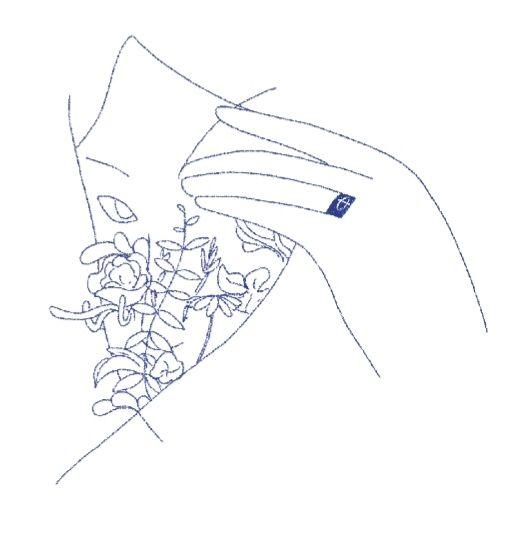
\includegraphics{images/contra.jpg}

  \bibliography{book.bib,packages.bib}

\end{document}
